\documentclass[a4paper,11pt]{article}
\usepackage[utf8]{inputenc}
\usepackage{graphicx}       % front image
\usepackage{hyperref}       % links and email
\usepackage[brazil]{babel} % linebreaks for english words
\usepackage{eurosym}
\usepackage{pbox}           % linebreaks in tables

% footnotes in tables
\usepackage{footnote}
\makesavenoteenv{tabular}

% auto update years
\usepackage{datenumber}
\newcounter{dateone}
\newcounter{datetwo}
\newcommand{\difftoday}[3]{%
      \setmydatenumber{dateone}{\the\year}{\the\month}{\the\day}%
      \setmydatenumber{datetwo}{#1}{#2}{#3}%
      \addtocounter{datetwo}{-\thedateone}%
      \the\numexpr-\thedatetwo/365\relax
}

% opening
\title{Plano de Negócio\\TerraCota}
\author{Álvaro Fernando\\Desenvolvedor - Gerente}

\begin{document}
\begin{titlepage}
    \centering
    \maketitle
    \thispagestyle{empty}   % discard page number
    
\includegraphics[width=10cm]{logo_inicial.jpg}
    \vfill
    {\raggedright
    NullPointer Corporation\\
    https://github.com/nullpointercorporation\\
    \href{mailto:nullpointercorporation@gmail.com}{nullpointercorporation@gmail.com}\\
    }
\end{titlepage}

\begin{abstract}
Este documento apresentará o plano de negócios para o desenvolvimento do jogo TerraCota, mostrando principalmente qual é o foco do desenvolvimento desse jogo, custos, público-alvo entre outros aspectos importantes para o desenvolvimento.

\end{abstract}

\pagebreak
\tableofcontents
\pagebreak

\section{Triângulo de Prioridades}
float
\begin{figure}[ht]
\centering
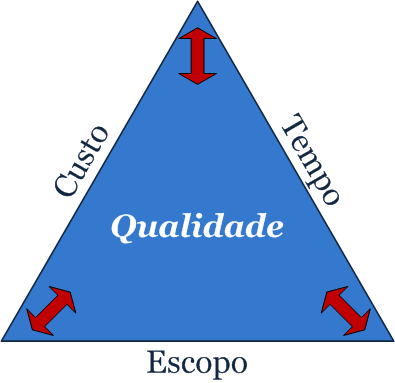
\includegraphics[width=5cm]{3_restricoes.png}
\caption{Triângulo de Prioridades}
\label{fig:restricoes}
\end{figure}

A figura acima apresenta o triângulo de prioridades com as três prioridades principais do projeto. O projeto estará focado no tempo e escopo, pois o custo total para realização do jogo será fixo e irrisório. \\
Com relação ao tempo o projeto terá uma duração de 4 meses, ou seja, o desenvolvimento deverá correr rápido para que a equipe consiga entregar o jogo no prazo estipulado, porém, a qualidade não pode ser deixada de lado e o grupo buscará a melhor qualidade possível. \\
Mesmo com o curto prazo de desenvolvimento o jogo deverá conter também muitas funcionalidades. Deverá conter ao menos 5 momentos jogáveis e completamente desenvolvidas para os usuários finais.

\section{Plataformas}

As plataformas suportadas, inicialmente, serão Windows e Linux.
O Linux possui um grande suporte de bibliotecas e ferramentas de desenvolvimento de software e o Windows possui uma grande base de usuários jogadores, fazendo com que ambas os sistemas operacionais se tornem alvos para o jogo.


\section{Público-alvo}
Pessoas acima de 10 anos, com capacidade de ler, escrever e interpretar signos, e interesse por Puzzles/Enigmas, RPGs e jogos de exploração.

\section{Estratégia de divulgação}

O jogo TerraCota será divulgado nas seguintes mídias:
\begin{itemize}
  \item Redes sociais:
  \begin{itemize}
    \item Divulgação nas timelines dos desenvolvedores
    \item Divulgação nos grupos de desenvolvimento de jogos independentes, exemplo Indie Developers Brasil, Boteco Gamer, GameDev-DF, etc.
  \end{itemize}
  \item Fóruns de jogos eletrônicos
    \begin{itemize}
      \item QUAIS?	 (TODO)
  \end{itemize}
  \item Steam Greenlight
\end{itemize}

\section{Recursos disponíveis}

Os recursos disponíveis para o desenvolvimento contam com uma equipe de sete pessoas, sendo três desenvolvedores, três artistas e um músico, também contam os equipamentos usados por cada membro da equipe. A seguir é apresentada uma tabela com os dados financeiros relacionados aos recursos disponíveis.

\begin{table}[h]
\begin{tabular}{|l|l|l|l|l}
\cline{1-4}
\multicolumn{1}{|c|}{\textbf{Recursos}} & \multicolumn{1}{c|}{\textbf{Quantidade}} & \multicolumn{1}{c|}{\textbf{Valor Unitário}} & \multicolumn{1}{c|}{\textbf{Valor Total}} &  \\ \cline{1-4}
Notebooks                               & 7                                        & R\$ 2.300,00                                  & R\$ 16.100,00                             &  \\ \cline{1-4}
Sublime Text 3                          & 3                                        & R\$ 212,10                                   & R\$ 636,30                                &  \\ \cline{1-4}
Linux                                   & 3                                        & R\$ 0,00                                     & R\$ 0,00                                  &  \\ \cline{1-4}
Windows 8                               & 4                                        & R\$ 359,00                                   & R\$ 1.436,00                              &  \\ \cline{1-4}
*Adobe Ilustrator CC                    & 3                                        & R\$ 176,00                                   & R\$ 528,00                                &  \\ \cline{1-4}
*Adobe Photoshop CC Fotografia          & 3                                        & R\$ 88,00                                    & R\$ 264,00                                &  \\ \cline{1-4}
Publicação na Steam Greenligth          & 1                                        & R\$ 304,12                                   & R\$ 304,12                                &  \\ \cline{1-4}
\multicolumn{3}{|c|}{\textbf{Total}}                                                                                              & R\$ 19.267,30                             &  \\ \cline{1-4}
\end{tabular}
\caption {Recursos de Hardware e Software}
\end{table}

\textit{* Os valores desses produtos são pagos por mês, a conta já converte o valor para 4 meses de uso.}
\\
\\
\\
\\
\\
\\

\begin{table}[h]
\begin{tabular}{|l|l|l|l|l}
\cline{1-4}
\multicolumn{1}{|c|}{\textbf{Recursos}} & \multicolumn{1}{c|}{\textbf{Quantidade}} & \multicolumn{1}{c|}{\textbf{Valor Hora}} & \multicolumn{1}{c|}{\textbf{Valor Total}} &  \\ \cline{1-4}
Desenvolvedor                           & 3                                        & R\$ 21,51                                & R\$ 41.299,20                             &  \\ \cline{1-4}
Designer Gráfico                        & 3                                        & R\$ 11,94                                & R\$ 2.2924,80                             &  \\ \cline{1-4}
Músico                                  & 1                                        & R\$ 8,35                                 & R\$ 5.344,00                              &  \\ \cline{1-4}
\multicolumn{3}{|c|}{\textbf{Total}}                                                                                          & R\$ 69.568,00                             &  \\ \cline{1-4}
\end{tabular}
\caption {Recursos Humanos}
\end{table}

\textit{* Todos os valores foram calculados considerando-se 40 horas de trabalho semanais em 4 meses de trabalho.}
\textit{Fonte de Pesquisa: \url{http://www.salariobr.com/}}
\\

Valor total do projeto: {\textbf{R\$ 88.835,30.}}

\section{Lucro esperado}

A equipe espera alcançar um lucros perto de 40\% em cima dos valores gastos para o desenvolvimento do jogo, para isso, é necessário se alcançar um valor em torno de R\$ 124.369,42 nas vendas, deixando assim todas as dívidas quitadas e mais R\$ 35.534,12 líquido.

\section{Número estimado de cópias a serem vendidas}

A seguir é apresentada uma tabela com determinados preços para o jogo e o número estimado de cópias que deveriam ser vendidas para se alcançar os lucros esperados, considerando também o custo do projeto. Os valores positivos são lucros além dos R\$ 124.369,42 (custo + lucro\_esperado). 

\begin{table}[h]
\begin{tabular}{|l|l|l|l|l}
\cline{1-4}
\multicolumn{1}{|c|}{\textbf{Valor do Jogo}} & \multicolumn{1}{c|}{\textbf{5k cópias vendidas}} & \multicolumn{1}{c|}{\textbf{10k cópias vendidas}} & \multicolumn{1}{c|}{\textbf{15k cópias vendidas}} &  \\ \cline{1-4}
R\$ 10,00                                    & R\$ -74.369,42                                        & R\$ -24.000,00                                        & R\$ 25.630,58                                     &  \\ \cline{1-4}
R\$ 15,00                                    & R\$ -49.369,42                                        & R\$ 25.630,58                                        & R\$ 100.630,58                                     &  \\ \cline{1-4}
R\$ 20,00                                    & R\$ -24.369,42                                       & R\$ 75.630,58                                        & R\$ 175.630,58                                     &  \\ \cline{1-4}
\end{tabular}
\caption{Valores alcançados de acordo com o valor do jogo}
\end{table}

\section{Projeção do número de cópias a serem vendidas para recuperar o
	    investimento e para se obter o lucro esperado}

Pode-se notar na tabela com os valores apresentados as opções possíveis para as vendas do jogo. Para quitar os gastos do projeto e se obter o lucro esperado com uma meta de vendas para 5 mil cópias, o jogo deverá ter um valor de R\$ 24,88. Com uma expectativa de 10 mil cópias vendidas já fica possível o valor de R\$ 12,44. E para um meta de 15 mil cópias, o valor seria R\$ 8,30.

\end{document}
